\chapter{Finite Differences}
Finite difference schemes are very much similar to trinomial tree options pricing, where each node is dependent on three other nodes with an up movement, a down movement, and a flat movement.
 
 \section{Finite Differences in Option Pricing}
The motivation behind the finite differencing is the application of the Black-Scholes Partial Differential Equation (PDE) framework (involving functions and their partial derivatives) whose price $S(t)$ is a function of
$f(S,t)$, with $r$ as the risk-free rate, $t$ as the time to maturity, and $\sigma$ as the volatility of the underlying security:

\begin{equation}
rf = \cfrac{\partial f}{\partial t} + rS\cfrac{\partial f}{\partial S} + \cfrac{1}{2} \sigma^2 S^2 \cfrac{\partial ^2 f}{\partial t^2}
\end{equation}

The finite difference technique tends to converge faster than lattices and approximates complex exotic options very well.
To solve a PDE by finite differences working backward in time, a discrete-time grid of size $M$ by $N$ is set up to reflect asset prices over a course of time, such that $S$ and
$t$ take on the following values at each point on the grid:

\begin{equation}
\begin{gathered}
S = 0, dS, 2dS, 3dS,\ldots, (M −1) dS, S_{max} \\
t = 0, dt, 2dt, 3dt,\ldots (N −1) dt, T
\end{gathered}
\end{equation}

It follows that by grid notation, $f_{i, j} = f (idS, jdt)$. $S_{max}$ is a suitably large asset price that cannot be reached by the maturity time, $T$. $dS$ and $dt$ are thus intervals between each node in the grid, incremented by price and time respectively. The terminal condition at expiration time $T$ for every value of $S$ is $\textrm{max}(S − K,0)$ for a call option with strike $K$ and $\textrm{max}(K − S,0)$ for a put option. The grid traverses backward from the terminal conditions, complying with the PDE while adhering to the boundary conditions of the grid, such as the payoff from an early exercise.

The boundary conditions are defined values at the extreme ends of the nodes, where $i=0$ and $i=N$ for every time at $t$. Values at the boundaries are used to calculate the values of all other lattice nodes iteratively using the PDE.

A visual representation of the grid is given by the following figure. As $i$ and $j$ increase from the top-left corner of the grid, the price $S$ tends toward $S_{max}$ (the maximum price possible) at the bottom-right corner of the grid:
A number of ways to approximate the PDE are as follows: 

\begin{itemize}
\item Forward difference:
\begin{equation}
\cfrac{\partial f}{\partial S} = \cfrac{f_{i+1,j} − f_{i,j}}{\partial S},\quad \cfrac{\partial f}{\partial t} = \cfrac{f_{i,j+1} − f_{i,j}}{\partial t}
\end{equation}

\item Backward difference:
\begin{equation}
	\cfrac{\partial f}{\partial S} = \cfrac{f_{i,j} − f_{i-1,j}}{\partial S},\quad \cfrac{\partial f}{\partial t} = \cfrac{f_{i,j} − f_{i,j-1}}{\partial t}
\end{equation}

\item Central or symmetric difference:
\begin{equation}
	\cfrac{\partial f}{\partial S} = \cfrac{f_{i+1,j} − f_{i-1,j}}{2\partial S},\quad \cfrac{\partial f}{\partial t} = \cfrac{f_{i,j+1} − f_{i,j-1}}{2\partial t}
\end{equation}

\item The second derivative:
\begin{equation}
	\cfrac{\partial^2 f}{\partial S^2} = \cfrac{f_{i+1,j} − 2f_{i,j} +  f_{i-1,j}}{2\partial S^2}
\end{equation}
\end{itemize}

Once we have the boundary conditions set up, we can now apply an iterative approach using the explicit, implicit, or Crank-Nicolson method.

\subsection{The Explicit Method}
The explicit method for approximating $f_{i, j}$ is given by:

\begin{equation}
rf_{i,j} = \cfrac{f_{i,j} − f_{i,j−1}}{dt} + ridS \cfrac{f_{i+1,j} − f_{i−1,j}}{2dS} +\cfrac{1}{2} \sigma^2 j^2 \cfrac{f_{i+1,j} + f_{i−1,j}}{dS^2}
\end{equation}

Here, it can be seen that the first difference is the backward difference with respect to $t$, the second difference is the central difference with respect to $S$, and the third difference is the second-order difference with respect to $S$. When we rearrange the terms, we have the following equation:

\begin{equation}
f_{i,j} =a^* f_{i-1,j+1} +b^* f_{i,j+1} +c^* f_{i+1,j+1}
\end{equation}
where $j=N−1,N−2,N−3,\ldots, 2,1,0$ and $i=1,2,3,\ldots, M−2,M−1$:

\begin{equation}
\begin{gathered}
a^* = \cfrac{1}{2}dt(\sigma^2 i^2 −ri)\\
b^* =1−dt(\sigma^2 i^2 −ri) \\
c^* = \cfrac{1}{2}dt(\sigma^2 i^2 +ri)
\end{gathered}	
\end{equation} 
 
The iterative approach of the explicit method can be visually represented by the following figure:

\begin{center}
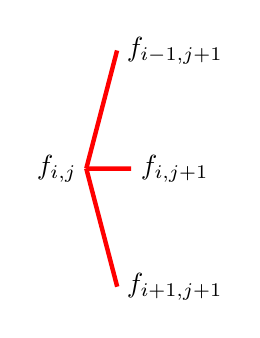
\begin{tikzpicture}
	[parent anchor=east,child anchor=west,grow=east]
	%\tikzstyle{every node}=[ball color=red,circle,text=white]
	\tikzstyle{edge from parent}=[draw,ultra thick,red]
	\node {$f_{i,j}$}
	child {node {$f_{i+1,j+1}$}}
	child {node {$f_{i,j+1}$}}
	child {node {$f_{i-1,j+1}$}};
\end{tikzpicture}
\end{center}

\subsection{\texttt{FiniteDifferences} class}
As we will be writing the explicit, implicit, and Crank-Nicolson methods of finite differences in \texttt{python}, let's write a parent class that can inherit the common properties and functions of all three methods.

We will create a class called \texttt{FiniteDifferences} that accepts and assigns all the required parameters in the constructor method.

\begin{codebox}
\begin{Verbatim}[commandchars=\\\{\}]
\PY{k+kn}{import} \PY{n+nn}{numpy} \PY{k}{as} \PY{n+nn}{np}
		
\PY{k}{class} \PY{n+nc}{FiniteDifferences}\PY{p}{:}
    \PY{k}{def} \PY{n+nf+fm}{\PYZus{}\PYZus{}init\PYZus{}\PYZus{}}\PY{p}{(}\PY{n+nb+bp}{self}\PY{p}{,} \PY{n}{S0}\PY{p}{,} \PY{n}{K}\PY{p}{,} \PY{n}{r}\PY{p}{,} \PY{n}{T}\PY{p}{,} \PY{n}{sigma}\PY{p}{,} \PY{n}{Smax}\PY{p}{,} \PY{n}{M}\PY{p}{,} \PY{n}{N}\PY{p}{,} \PY{n}{is\PYZus{}call} \PY{o}{=} \PY{k+kc}{True}\PY{p}{)}\PY{p}{:}
        \PY{n+nb+bp}{self}\PY{o}{.}\PY{n}{S0} \PY{o}{=} \PY{n}{S0}
        \PY{n+nb+bp}{self}\PY{o}{.}\PY{n}{K} \PY{o}{=} \PY{n}{K}
        \PY{n+nb+bp}{self}\PY{o}{.}\PY{n}{r} \PY{o}{=} \PY{n}{r}
        \PY{n+nb+bp}{self}\PY{o}{.}\PY{n}{T} \PY{o}{=} \PY{n}{T}
        \PY{n+nb+bp}{self}\PY{o}{.}\PY{n}{sigma} \PY{o}{=} \PY{n}{sigma}
        \PY{n+nb+bp}{self}\PY{o}{.}\PY{n}{Smax} \PY{o}{=} \PY{n}{Smax}
        \PY{n+nb+bp}{self}\PY{o}{.}\PY{n}{M}\PY{p}{,} \PY{n+nb+bp}{self}\PY{o}{.}\PY{n}{N} \PY{o}{=} \PY{n+nb}{int}\PY{p}{(}\PY{n}{M}\PY{p}{)}\PY{p}{,} \PY{n+nb}{int}\PY{p}{(}\PY{n}{N}\PY{p}{)}
        \PY{n+nb+bp}{self}\PY{o}{.}\PY{n}{is\PYZus{}call} \PY{o}{=} \PY{n}{is\PYZus{}call}
        \PY{n+nb+bp}{self}\PY{o}{.}\PY{n}{dS} \PY{o}{=} \PY{n}{Smax} \PY{o}{/} \PY{n+nb}{float}\PY{p}{(}\PY{n+nb+bp}{self}\PY{o}{.}\PY{n}{M}\PY{p}{)}
        \PY{n+nb+bp}{self}\PY{o}{.}\PY{n}{dt} \PY{o}{=} \PY{n}{T} \PY{o}{/} \PY{n+nb}{float}\PY{p}{(}\PY{n+nb+bp}{self}\PY{o}{.}\PY{n}{N}\PY{p}{)}
        \PY{n+nb+bp}{self}\PY{o}{.}\PY{n}{i\PYZus{}values} \PY{o}{=} \PY{n}{np}\PY{o}{.}\PY{n}{arange}\PY{p}{(}\PY{n+nb+bp}{self}\PY{o}{.}\PY{n}{M}\PY{p}{)}
        \PY{n+nb+bp}{self}\PY{o}{.}\PY{n}{j\PYZus{}values} \PY{o}{=} \PY{n}{np}\PY{o}{.}\PY{n}{arange}\PY{p}{(}\PY{n+nb+bp}{self}\PY{o}{.}\PY{n}{N}\PY{p}{)}
        \PY{n+nb+bp}{self}\PY{o}{.}\PY{n}{grid} \PY{o}{=} \PY{n}{np}\PY{o}{.}\PY{n}{zeros}\PY{p}{(}\PY{n}{shape}\PY{o}{=}\PY{p}{(}\PY{n+nb+bp}{self}\PY{o}{.}\PY{n}{M}\PY{o}{+}\PY{l+m+mi}{1}\PY{p}{,} \PY{n+nb+bp}{self}\PY{o}{.}\PY{n}{N}\PY{o}{+}\PY{l+m+mi}{1}\PY{p}{)}\PY{p}{)} 
        \PY{n+nb+bp}{self}\PY{o}{.}\PY{n}{boundary\PYZus{}conds} \PY{o}{=} \PY{n}{np}\PY{o}{.}\PY{n}{linspace}\PY{p}{(}\PY{l+m+mi}{0}\PY{p}{,} \PY{n}{Smax}\PY{p}{,} \PY{n+nb+bp}{self}\PY{o}{.}\PY{n}{M}\PY{o}{+}\PY{l+m+mi}{1}\PY{p}{)}
		
    \PY{k}{def} \PY{n+nf}{\PYZus{}setup\PYZus{}boundary\PYZus{}conditions\PYZus{}}\PY{p}{(}\PY{n+nb+bp}{self}\PY{p}{)}\PY{p}{:}
        \PY{k}{pass}
		
    \PY{k}{def} \PY{n+nf}{\PYZus{}setup\PYZus{}coefficients\PYZus{}}\PY{p}{(}\PY{n+nb+bp}{self}\PY{p}{)}\PY{p}{:}
        \PY{k}{pass}
		
    \PY{k}{def} \PY{n+nf}{\PYZus{}traverse\PYZus{}grid\PYZus{}}\PY{p}{(}\PY{n+nb+bp}{self}\PY{p}{)}\PY{p}{:}
        \PY{k}{pass}
		
    \PY{k}{def} \PY{n+nf}{\PYZus{}interpolate\PYZus{}}\PY{p}{(}\PY{n+nb+bp}{self}\PY{p}{)}\PY{p}{:}
        \PY{k}{return} \PY{n}{np}\PY{o}{.}\PY{n}{interp}\PY{p}{(}\PY{n+nb+bp}{self}\PY{o}{.}\PY{n}{S0}\PY{p}{,} \PY{n+nb+bp}{self}\PY{o}{.}\PY{n}{boundary\PYZus{}conds}\PY{p}{,} \PY{n+nb+bp}{self}\PY{o}{.}\PY{n}{grid}\PY{p}{[}\PY{p}{:}\PY{p}{,} \PY{l+m+mi}{0}\PY{p}{]}\PY{p}{)}
		
    \PY{k}{def} \PY{n+nf}{price}\PY{p}{(}\PY{n+nb+bp}{self}\PY{p}{)}\PY{p}{:} 
        \PY{n+nb+bp}{self}\PY{o}{.}\PY{n}{\PYZus{}setup\PYZus{}boundary\PYZus{}conditions\PYZus{}}\PY{p}{(}\PY{p}{)} 
        \PY{n+nb+bp}{self}\PY{o}{.}\PY{n}{\PYZus{}setup\PYZus{}coefficients\PYZus{}}\PY{p}{(}\PY{p}{)} 
        \PY{n+nb+bp}{self}\PY{o}{.}\PY{n}{\PYZus{}traverse\PYZus{}grid\PYZus{}}\PY{p}{(}\PY{p}{)}
        \PY{k}{return} \PY{n+nb+bp}{self}\PY{o}{.}\PY{n}{\PYZus{}interpolate\PYZus{}}\PY{p}{(}\PY{p}{)}
\end{Verbatim}
\end{codebox}

All of these methods are protected methods and may be overwritten by derived classes. The pass keyword simply does nothing; the derived classes will provide specific implementations of these functions.

\subsubsection{\texttt{FDExplicitEu} class}

The \texttt{python} implementation of finite differences by the explicit method is given in the following \texttt{FDExplicitEu} class, which inherits from the \texttt{FiniteDifferences} class and overrides the required implementation methods.

\begin{codebox}
\begin{Verbatim}[commandchars=\\\{\}]
\PY{k+kn}{import} \PY{n+nn}{numpy} \PY{k}{as} \PY{n+nn}{np}
		
\PY{k}{class} \PY{n+nc}{FDExplicitEu}\PY{p}{(}\PY{n}{FiniteDifferences}\PY{p}{)}\PY{p}{:}
    \PY{k}{def} \PY{n+nf}{\PYZus{}setup\PYZus{}boundary\PYZus{}conditions\PYZus{}}\PY{p}{(}\PY{n+nb+bp}{self}\PY{p}{)}\PY{p}{:} 
        \PY{k}{if} \PY{n+nb+bp}{self}\PY{o}{.}\PY{n}{is\PYZus{}call}\PY{p}{:}
            \PY{n+nb+bp}{self}\PY{o}{.}\PY{n}{grid}\PY{p}{[}\PY{p}{:}\PY{p}{,} \PY{o}{\PYZhy{}}\PY{l+m+mi}{1}\PY{p}{]} \PY{o}{=} \PY{n}{np}\PY{o}{.}\PY{n}{maximum}\PY{p}{(}\PY{n+nb+bp}{self}\PY{o}{.}\PY{n}{boundary\PYZus{}conds} \PY{o}{\PYZhy{}} \PY{n+nb+bp}{self}\PY{o}{.}\PY{n}{K}\PY{p}{,} \PY{l+m+mi}{0}\PY{p}{)}
            \PY{n+nb+bp}{self}\PY{o}{.}\PY{n}{grid}\PY{p}{[}\PY{o}{\PYZhy{}}\PY{l+m+mi}{1}\PY{p}{,} \PY{p}{:}\PY{o}{\PYZhy{}}\PY{l+m+mi}{1}\PY{p}{]} \PY{o}{=} \PY{p}{(}\PY{n+nb+bp}{self}\PY{o}{.}\PY{n}{Smax} \PY{o}{\PYZhy{}} \PY{n+nb+bp}{self}\PY{o}{.}\PY{n}{K}\PY{p}{)} \PY{o}{*} 
                \PY{n}{np}\PY{o}{.}\PY{n}{exp}\PY{p}{(}\PY{o}{\PYZhy{}}\PY{n+nb+bp}{self}\PY{o}{.}\PY{n}{r} \PY{o}{*} \PY{n+nb+bp}{self}\PY{o}{.}\PY{n}{dt} \PY{o}{*} \PY{p}{(}\PY{n+nb+bp}{self}\PY{o}{.}\PY{n}{N}\PY{o}{\PYZhy{}}\PY{n+nb+bp}{self}\PY{o}{.}\PY{n}{j\PYZus{}values}\PY{p}{)}\PY{p}{)}
        \PY{k}{else}\PY{p}{:}
            \PY{n+nb+bp}{self}\PY{o}{.}\PY{n}{grid}\PY{p}{[}\PY{p}{:}\PY{p}{,} \PY{o}{\PYZhy{}}\PY{l+m+mi}{1}\PY{p}{]} \PY{o}{=} \PY{n}{np}\PY{o}{.}\PY{n}{maximum}\PY{p}{(}\PY{n+nb+bp}{self}\PY{o}{.}\PY{n}{K}\PY{o}{\PYZhy{}}\PY{n+nb+bp}{self}\PY{o}{.}\PY{n}{boundary\PYZus{}conds}\PY{p}{,} \PY{l+m+mi}{0}\PY{p}{)} 
            \PY{n+nb+bp}{self}\PY{o}{.}\PY{n}{grid}\PY{p}{[}\PY{l+m+mi}{0}\PY{p}{,} \PY{p}{:}\PY{o}{\PYZhy{}}\PY{l+m+mi}{1}\PY{p}{]} \PY{o}{=} \PY{p}{(}\PY{n+nb+bp}{self}\PY{o}{.}\PY{n}{K} \PY{o}{\PYZhy{}} \PY{n+nb+bp}{self}\PY{o}{.}\PY{n}{Smax}\PY{p}{)} \PY{o}{*} \PY{n}{np}\PY{o}{.}\PY{n}{exp}\PY{p}{(}\PY{o}{\PYZhy{}}\PY{n+nb+bp}{self}\PY{o}{.}\PY{n}{r} 
                \PY{o}{*} \PY{n+nb+bp}{self}\PY{o}{.}\PY{n}{dt} \PY{o}{*} \PY{p}{(}\PY{n+nb+bp}{self}\PY{o}{.}\PY{n}{N}\PY{o}{\PYZhy{}}\PY{n+nb+bp}{self}\PY{o}{.}\PY{n}{j\PYZus{}values}\PY{p}{)}\PY{p}{)}
		
    \PY{k}{def} \PY{n+nf}{\PYZus{}setup\PYZus{}coefficients\PYZus{}}\PY{p}{(}\PY{n+nb+bp}{self}\PY{p}{)}\PY{p}{:}
        \PY{n+nb+bp}{self}\PY{o}{.}\PY{n}{a} \PY{o}{=} \PY{l+m+mf}{0.5}\PY{o}{*}\PY{n+nb+bp}{self}\PY{o}{.}\PY{n}{dt}\PY{o}{*}\PY{p}{(}\PY{p}{(}\PY{n+nb+bp}{self}\PY{o}{.}\PY{n}{sigma}\PY{o}{*}\PY{o}{*}\PY{l+m+mi}{2}\PY{p}{)} \PY{o}{*} \PY{p}{(}\PY{n+nb+bp}{self}\PY{o}{.}\PY{n}{i\PYZus{}values}\PY{o}{*}\PY{o}{*}\PY{l+m+mi}{2}\PY{p}{)} 
                 \PY{o}{\PYZhy{}} \PY{n+nb+bp}{self}\PY{o}{.}\PY{n}{r}\PY{o}{*}\PY{n+nb+bp}{self}\PY{o}{.}\PY{n}{i\PYZus{}values}\PY{p}{)} 
        \PY{n+nb+bp}{self}\PY{o}{.}\PY{n}{b} \PY{o}{=} \PY{l+m+mi}{1} \PY{o}{\PYZhy{}} \PY{n+nb+bp}{self}\PY{o}{.}\PY{n}{dt}\PY{o}{*}\PY{p}{(}\PY{p}{(}\PY{n+nb+bp}{self}\PY{o}{.}\PY{n}{sigma}\PY{o}{*}\PY{o}{*}\PY{l+m+mi}{2}\PY{p}{)} \PY{o}{*} \PY{p}{(}\PY{n+nb+bp}{self}\PY{o}{.}\PY{n}{i\PYZus{}values}\PY{o}{*}\PY{o}{*}\PY{l+m+mi}{2}\PY{p}{)} 
                 \PY{o}{+} \PY{n+nb+bp}{self}\PY{o}{.}\PY{n}{r}\PY{p}{)}
        \PY{n+nb+bp}{self}\PY{o}{.}\PY{n}{c} \PY{o}{=} \PY{l+m+mf}{0.5}\PY{o}{*}\PY{n+nb+bp}{self}\PY{o}{.}\PY{n}{dt}\PY{o}{*}\PY{p}{(}\PY{p}{(}\PY{n+nb+bp}{self}\PY{o}{.}\PY{n}{sigma}\PY{o}{*}\PY{o}{*}\PY{l+m+mi}{2}\PY{p}{)} \PY{o}{*} \PY{p}{(}\PY{n+nb+bp}{self}\PY{o}{.}\PY{n}{i\PYZus{}values}\PY{o}{*}\PY{o}{*}\PY{l+m+mi}{2}\PY{p}{)} 
                 \PY{o}{+} \PY{n+nb+bp}{self}\PY{o}{.}\PY{n}{r}\PY{o}{*}\PY{n+nb+bp}{self}\PY{o}{.}\PY{n}{i\PYZus{}values}\PY{p}{)}
		
    \PY{k}{def} \PY{n+nf}{\PYZus{}traverse\PYZus{}grid\PYZus{}}\PY{p}{(}\PY{n+nb+bp}{self}\PY{p}{)}\PY{p}{:}
        \PY{k}{for} \PY{n}{j} \PY{o+ow}{in} \PY{n+nb}{reversed}\PY{p}{(}\PY{n+nb+bp}{self}\PY{o}{.}\PY{n}{j\PYZus{}values}\PY{p}{)}\PY{p}{:}
            \PY{k}{for} \PY{n}{i} \PY{o+ow}{in} \PY{n+nb}{range}\PY{p}{(}\PY{n+nb+bp}{self}\PY{o}{.}\PY{n}{M}\PY{p}{)}\PY{p}{[}\PY{l+m+mi}{2}\PY{p}{:}\PY{p}{]}\PY{p}{:}
                \PY{n+nb+bp}{self}\PY{o}{.}\PY{n}{grid}\PY{p}{[}\PY{n}{i}\PY{p}{,}\PY{n}{j}\PY{p}{]} \PY{o}{=} \PY{n+nb+bp}{self}\PY{o}{.}\PY{n}{a}\PY{p}{[}\PY{n}{i}\PY{p}{]}\PY{o}{*}\PY{n+nb+bp}{self}\PY{o}{.}\PY{n}{grid}\PY{p}{[}\PY{n}{i}\PY{o}{\PYZhy{}}\PY{l+m+mi}{1}\PY{p}{,}\PY{n}{j}\PY{o}{+}\PY{l+m+mi}{1}\PY{p}{]} \PY{o}{+} 
                                 \PY{n+nb+bp}{self}\PY{o}{.}\PY{n}{b}\PY{p}{[}\PY{n}{i}\PY{p}{]}\PY{o}{*}\PY{n+nb+bp}{self}\PY{o}{.}\PY{n}{grid}\PY{p}{[}\PY{n}{i}\PY{p}{,}\PY{n}{j}\PY{o}{+}\PY{l+m+mi}{1}\PY{p}{]} \PY{o}{+} 
                                 \PY{n+nb+bp}{self}\PY{o}{.}\PY{n}{c}\PY{p}{[}\PY{n}{i}\PY{p}{]}\PY{o}{*}\PY{n+nb+bp}{self}\PY{o}{.}\PY{n}{grid}\PY{p}{[}\PY{n}{i}\PY{o}{+}\PY{l+m+mi}{1}\PY{p}{,}\PY{n}{j}\PY{o}{+}\PY{l+m+mi}{1}\PY{p}{]}
\end{Verbatim}
\end{codebox}

On completion of traversing the grid structure, the first column contains the present value of the initial asset prices at t=0. The \texttt{interp} function of \texttt{numpy} is used to perform a linear interpolation to approximate the option value.

Besides using linear interpolation as the most common choice for the interpolation method, the other methods such as the spline or cubic may be used to approximate the option value.
Consider the example of an European put option. The underlying stock price is \$50 with a volatility of 0.4. The strike price of the put option is \$50 with an expiration time of 5 months. The risk-free rate is 10 percent.
We can price the option using the explicit method with a $S_{max}$ value of 100, an M value of 1000, and a N 

\begin{codebox}
\begin{Verbatim}[commandchars=\\\{\}]
\PY{n}{option} \PY{o}{=} \PY{n}{FDExplicitEu}\PY{p}{(}\PY{l+m+mi}{50}\PY{p}{,} \PY{l+m+mi}{50}\PY{p}{,} \PY{l+m+mf}{0.1}\PY{p}{,} \PY{l+m+mf}{5.}\PY{o}{/}\PY{l+m+mf}{12.}\PY{p}{,} \PY{l+m+mf}{0.4}\PY{p}{,} \PY{l+m+mi}{100}\PY{p}{,} \PY{l+m+mi}{100}\PY{p}{,} \PY{l+m+mi}{1000}\PY{p}{,} \PY{k+kc}{False}\PY{p}{)}
\PY{n+nb}{print} \PY{p}{(}\PY{n}{option}\PY{o}{.}\PY{n}{price}\PY{p}{(}\PY{p}{)}\PY{p}{)}

4.072882278148043
\end{Verbatim}
\end{codebox}

What happens when other values of M and N are chosen improperly?

\begin{codebox}
\begin{Verbatim}[commandchars=\\\{\}]
\PY{n}{option} \PY{o}{=} \PY{n}{FDExplicitEu}\PY{p}{(}\PY{l+m+mi}{50}\PY{p}{,} \PY{l+m+mi}{50}\PY{p}{,} \PY{l+m+mf}{0.1}\PY{p}{,} \PY{l+m+mf}{5.}\PY{o}{/}\PY{l+m+mf}{12.}\PY{p}{,} \PY{l+m+mf}{0.4}\PY{p}{,} \PY{l+m+mi}{100}\PY{p}{,} \PY{l+m+mi}{100}\PY{p}{,} \PY{l+m+mi}{100}\PY{p}{,} \PY{k+kc}{False}\PY{p}{)}
\PY{n+nb}{print} \PY{p}{(}\PY{n}{option}\PY{o}{.}\PY{n}{price}\PY{p}{(}\PY{p}{)}\PY{p}{)}

-1.6291077072251005e+53
\end{Verbatim}
\end{codebox}

It appears that the explicit method of the finite difference scheme suffers from instability problems.

\subsubsection{\texttt{FDImplicitEu} class}

The instability problem of the explicit method can be overcome using the forward difference with respect to time. The implicit method for approximating $f_{i, j}$ is given by:

\begin{equation}
	rf_{i,j} = \cfrac{f_{i,j} − f_{i,j−1}}{dt} + ridS \cfrac{f_{i+1,j} − f_{i−1,j}}{2dS} +\cfrac{1}{2} \sigma^2 j^2 \cfrac{f_{i+1,j} + f_{i−1,j}}{dS^2}
\end{equation}

Here, it can be seen that the only difference between the implicit and explicit approximating scheme lies in the first difference, where the forward difference with respect to $t$ is used in the implicit scheme. When we rearrange the terms, we have the following expression:

\begin{equation}
	f_{i,j+1} = a_i f_{i-1,j} +b_i f_{i,j} +c_i f_{i+1,j}
\end{equation}
where $j=N−1,N−2,N−3,\ldots, 2,1,0$ and $i=1,2,3,\ldots, M−1$:

\begin{equation}
	\begin{gathered}
		a_i = \cfrac{1}{2}dt(ri-\sigma^2 i^2)\\
		b_i =1+dt(ri+\sigma^2 i^2) \\
		c_i = -\cfrac{1}{2}+dt(\sigma^2 i^2 + ri)
	\end{gathered}	
\end{equation} 

The iterative approach of the explicit method can be visually represented by the following figure:

\begin{center}
	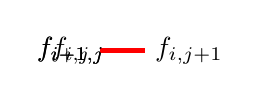
\begin{tikzpicture}
		[parent anchor=east,child anchor=west,grow=east]
		%\tikzstyle{every node}=[ball color=red,circle,text=white]
		\tikzstyle{edge from parent}=[draw,ultra thick,red]
		\node {$f_{i+1,j}$}
		 node {$f_{i,j}$}
			child {node {$f_{i,j+1}$}}
		 node {$f_{i-1,j}$};
	\end{tikzpicture}
\end{center}

From the figure, it is intuitive to note that values of $j + 1$ are required to be computed before they can be used in the next iterative step, as the grid traverses backward.
In the implicit scheme, the grid can be thought of as representing a system of linear equations at each iteration, as follows:

\begin{equation*}
\begin{bmatrix}
b_1    & c_1 & 0   & \cdots & 0 & 0 \\
a_2    & b_2 & c_2 & \cdots & 0 & 0 \\
0      & 0   & b_3 & \cdots & 0 & 0 \\
\vdots & \vdots & \vdots & \ddots & \vdots & \vdots \\
0   & 0 & 0 & a_{M-2} & b_{M-2} & c_{M-2} \\
0   & 0 & 0 & \cdots & a_{M-1} & b_{M-1}
\end{bmatrix}
\begin{bmatrix} 
	f_{1,j}\\
	f_{2,j}\\
	f_{3,j}\\
	\vdots\\
	f_{M-2,j}\\
	f_{M-1,j}\\
\end{bmatrix} +
\begin{bmatrix}
a_1 f_{0,j}\\
0\\
0\\
\vdots\\
0\\
c_{M-1}f_{M,j}\\
\end{bmatrix} =
\begin{bmatrix} 
f_{1,j+1}\\
f_{2,j+1}\\
f_{3,j+1}\\
\vdots\\
f_{M-2,j+1}\\
f_{M-1,j+1}\\
\end{bmatrix}
\end{equation*}
\noindent
By rearranging the terms, we get the following equation:
\begin{equation*}
\begin{bmatrix}
b_1    & c_1 & 0   & \cdots & 0 & 0 \\
a_2    & b_2 & c_2 & \cdots & 0 & 0 \\
0      & 0   & b_3 & \cdots & 0 & 0 \\
\vdots & \vdots & \vdots & \ddots & \vdots & \vdots \\
0   & 0 & 0 & a_{M-2} & b_{M-2} & c_{M-2} \\
0   & 0 & 0 & \cdots & a_{M-1} & b_{M-1}
\end{bmatrix}
\begin{bmatrix}
f_{1,j}\\
f_{2,j}\\
f_{3,j}\\
\vdots\\
f_{M-2,j}\\
f_{M-1,j}
\end{bmatrix} = 
\begin{bmatrix}
f_{1,j+1}\\
f_{2,j+1}\\
f_{3,j+1}\\
\vdots\\
f_{M-2,j+1}\\
f_{M-1,j+1}
\end{bmatrix} - 
\begin{bmatrix}
a_1 f_{0,j}\\
0\\
0\\
\vdots\\
0\\
c_{M-1}f_{M,j}
\end{bmatrix}
\end{equation*}

The linear system of equations can be represented in the form of $[A]x = [B]$, where we want to solve for values of $x$ in each iteration. Since the matrix $[A]$ is tri-diagonal, we can use the LU factorization, where $[A]=[L][U]$, for faster computation. 

The \texttt{python} implementation of the implicit scheme is given in the following \texttt{FDImplicitEu} class. We can inherit the implementation of the explicit method from the \texttt{FDExplicitEu} class discussed earlier and override the necessary methods of interest:

\begin{codebox}
\begin{Verbatim}[commandchars=\\\{\}]
\PY{k+kn}{import} \PY{n+nn}{scipy}\PY{n+nn}{.}\PY{n+nn}{linalg} \PY{k}{as} \PY{n+nn}{linalg}
		
\PY{k}{class} \PY{n+nc}{FDImplicitEu}\PY{p}{(}\PY{n}{FDExplicitEu}\PY{p}{)}\PY{p}{:}
    \PY{k}{def} \PY{n+nf}{\PYZus{}setup\PYZus{}coefficients\PYZus{}}\PY{p}{(}\PY{n+nb+bp}{self}\PY{p}{)}\PY{p}{:}
        \PY{n+nb+bp}{self}\PY{o}{.}\PY{n}{a} \PY{o}{=} \PY{l+m+mf}{0.5}\PY{o}{*}\PY{p}{(}\PY{n+nb+bp}{self}\PY{o}{.}\PY{n}{r}\PY{o}{*}\PY{n+nb+bp}{self}\PY{o}{.}\PY{n}{dt}\PY{o}{*}\PY{n+nb+bp}{self}\PY{o}{.}\PY{n}{i\PYZus{}values} \PY{o}{\PYZhy{}} \PY{p}{(}\PY{n+nb+bp}{self}\PY{o}{.}\PY{n}{sigma}\PY{o}{*}\PY{o}{*}\PY{l+m+mi}{2}\PY{p}{)}\PY{o}{*}\PY{n+nb+bp}{self}\PY{o}{.}\PY{n}{dt}\PY{o}{*}\PY{p}{(}\PY{n+nb+bp}{self}\PY{o}{.}\PY{n}{i\PYZus{}values}\PY{o}{*}\PY{o}{*}\PY{l+m+mi}{2}\PY{p}{)}\PY{p}{)} 
        \PY{n+nb+bp}{self}\PY{o}{.}\PY{n}{b} \PY{o}{=} \PY{l+m+mi}{1} \PY{o}{+} \PY{p}{(}\PY{n+nb+bp}{self}\PY{o}{.}\PY{n}{sigma}\PY{o}{*}\PY{o}{*}\PY{l+m+mi}{2}\PY{p}{)}\PY{o}{*}\PY{n+nb+bp}{self}\PY{o}{.}\PY{n}{dt}\PY{o}{*}\PY{p}{(}\PY{n+nb+bp}{self}\PY{o}{.}\PY{n}{i\PYZus{}values}\PY{o}{*}\PY{o}{*}\PY{l+m+mi}{2}\PY{p}{)} \PY{o}{+} \PY{n+nb+bp}{self}\PY{o}{.}\PY{n}{r}\PY{o}{*}\PY{n+nb+bp}{self}\PY{o}{.}\PY{n}{dt} 
        \PY{n+nb+bp}{self}\PY{o}{.}\PY{n}{c} \PY{o}{=} \PY{o}{\PYZhy{}}\PY{l+m+mf}{0.5}\PY{o}{*}\PY{p}{(}\PY{n+nb+bp}{self}\PY{o}{.}\PY{n}{r} \PY{o}{*} \PY{n+nb+bp}{self}\PY{o}{.}\PY{n}{dt}\PY{o}{*}\PY{n+nb+bp}{self}\PY{o}{.}\PY{n}{i\PYZus{}values} \PY{o}{+} \PY{p}{(}\PY{n+nb+bp}{self}\PY{o}{.}\PY{n}{sigma}\PY{o}{*}\PY{o}{*}\PY{l+m+mi}{2}\PY{p}{)}\PY{o}{*}\PY{n+nb+bp}{self}\PY{o}{.}\PY{n}{dt}\PY{o}{*}\PY{p}{(}\PY{n+nb+bp}{self}\PY{o}{.}\PY{n}{i\PYZus{}values}\PY{o}{*}\PY{o}{*}\PY{l+m+mi}{2}\PY{p}{)}\PY{p}{)} 
        \PY{n+nb+bp}{self}\PY{o}{.}\PY{n}{coeffs} \PY{o}{=} \PY{n}{np}\PY{o}{.}\PY{n}{diag}\PY{p}{(}\PY{n+nb+bp}{self}\PY{o}{.}\PY{n}{a}\PY{p}{[}\PY{l+m+mi}{2}\PY{p}{:}\PY{n+nb+bp}{self}\PY{o}{.}\PY{n}{M}\PY{p}{]}\PY{p}{,} \PY{o}{\PYZhy{}}\PY{l+m+mi}{1}\PY{p}{)} \PY{o}{+} \PY{n}{np}\PY{o}{.}\PY{n}{diag}\PY{p}{(}\PY{n+nb+bp}{self}\PY{o}{.}\PY{n}{b}\PY{p}{[}\PY{l+m+mi}{1}\PY{p}{:}\PY{n+nb+bp}{self}\PY{o}{.}\PY{n}{M}\PY{p}{]}\PY{p}{)} \PY{o}{+} \PY{n}{np}\PY{o}{.}\PY{n}{diag}\PY{p}{(}\PY{n+nb+bp}{self}\PY{o}{.}\PY{n}{c}\PY{p}{[}\PY{l+m+mi}{1}\PY{p}{:}\PY{n+nb+bp}{self}\PY{o}{.}\PY{n}{M}\PY{o}{\PYZhy{}}\PY{l+m+mi}{1}\PY{p}{]}\PY{p}{,} \PY{l+m+mi}{1}\PY{p}{)}
		
    \PY{k}{def} \PY{n+nf}{\PYZus{}traverse\PYZus{}grid\PYZus{}}\PY{p}{(}\PY{n+nb+bp}{self}\PY{p}{)}\PY{p}{:}
        \PY{n}{P}\PY{p}{,} \PY{n}{L}\PY{p}{,} \PY{n}{U} \PY{o}{=} \PY{n}{linalg}\PY{o}{.}\PY{n}{lu}\PY{p}{(}\PY{n+nb+bp}{self}\PY{o}{.}\PY{n}{coeffs}\PY{p}{)}
        \PY{n}{aux} \PY{o}{=} \PY{n}{np}\PY{o}{.}\PY{n}{zeros}\PY{p}{(}\PY{n+nb+bp}{self}\PY{o}{.}\PY{n}{M}\PY{o}{\PYZhy{}}\PY{l+m+mi}{1}\PY{p}{)}
        \PY{k}{for} \PY{n}{j} \PY{o+ow}{in} \PY{n+nb}{reversed}\PY{p}{(}\PY{n+nb}{range}\PY{p}{(}\PY{n+nb+bp}{self}\PY{o}{.}\PY{n}{N}\PY{p}{)}\PY{p}{)}\PY{p}{:}
            \PY{n}{aux}\PY{p}{[}\PY{l+m+mi}{0}\PY{p}{]} \PY{o}{=} \PY{n}{np}\PY{o}{.}\PY{n}{dot}\PY{p}{(}\PY{o}{\PYZhy{}}\PY{n+nb+bp}{self}\PY{o}{.}\PY{n}{a}\PY{p}{[}\PY{l+m+mi}{1}\PY{p}{]}\PY{p}{,} \PY{n+nb+bp}{self}\PY{o}{.}\PY{n}{grid}\PY{p}{[}\PY{l+m+mi}{0}\PY{p}{,} \PY{n}{j}\PY{p}{]}\PY{p}{)}
            \PY{n}{x1} \PY{o}{=} \PY{n}{linalg}\PY{o}{.}\PY{n}{solve}\PY{p}{(}\PY{n}{L}\PY{p}{,} \PY{n+nb+bp}{self}\PY{o}{.}\PY{n}{grid}\PY{p}{[}\PY{l+m+mi}{1}\PY{p}{:}\PY{n+nb+bp}{self}\PY{o}{.}\PY{n}{M}\PY{p}{,} \PY{n}{j}\PY{o}{+}\PY{l+m+mi}{1}\PY{p}{]}\PY{o}{+}\PY{n}{aux}\PY{p}{)} 
            \PY{n}{x2} \PY{o}{=} \PY{n}{linalg}\PY{o}{.}\PY{n}{solve}\PY{p}{(}\PY{n}{U}\PY{p}{,} \PY{n}{x1}\PY{p}{)}
            \PY{n+nb+bp}{self}\PY{o}{.}\PY{n}{grid}\PY{p}{[}\PY{l+m+mi}{1}\PY{p}{:}\PY{n+nb+bp}{self}\PY{o}{.}\PY{n}{M}\PY{p}{,} \PY{n}{j}\PY{p}{]} \PY{o}{=} \PY{n}{x2}
\end{Verbatim}
\end{codebox}

Using the same example as with the explicit scheme, we can price an European put option using the implicit scheme:

\begin{codebox}
\begin{Verbatim}[commandchars=\\\{\}]
\PY{n}{option} \PY{o}{=} \PY{n}{FDImplicitEu}\PY{p}{(}\PY{l+m+mi}{50}\PY{p}{,} \PY{l+m+mi}{50}\PY{p}{,} \PY{l+m+mf}{0.1}\PY{p}{,} \PY{l+m+mf}{5.}\PY{o}{/}\PY{l+m+mf}{12.}\PY{p}{,} \PY{l+m+mf}{0.4}\PY{p}{,} \PY{l+m+mi}{100}\PY{p}{,} \PY{l+m+mi}{100}\PY{p}{,} \PY{l+m+mi}{100}\PY{p}{,} \PY{k+kc}{False}\PY{p}{)}
\PY{n+nb}{print} \PY{p}{(}\PY{n}{option}\PY{o}{.}\PY{n}{price}\PY{p}{(}\PY{p}{)}\PY{p}{)}

4.065801939431454

\PY{n}{option} \PY{o}{=} \PY{n}{FDImplicitEu}\PY{p}{(}\PY{l+m+mi}{50}\PY{p}{,} \PY{l+m+mi}{50}\PY{p}{,} \PY{l+m+mf}{0.1}\PY{p}{,} \PY{l+m+mf}{5.}\PY{o}{/}\PY{l+m+mf}{12.}\PY{p}{,} \PY{l+m+mf}{0.4}\PY{p}{,} \PY{l+m+mi}{100}\PY{p}{,} \PY{l+m+mi}{100}\PY{p}{,} \PY{l+m+mi}{1000}\PY{p}{,} \PY{k+kc}{False}\PY{p}{)}
\PY{n+nb}{print} \PY{p}{(}\PY{n}{option}\PY{o}{.}\PY{n}{price}\PY{p}{(}\PY{p}{)}\PY{p}{)}

4.071594188049893
\end{Verbatim}
\end{codebox}

Given the current parameters and input data, it is observed that there are no stability issues with the implicit scheme.

\subsubsection{The Crank-Nicolson Method}
Another way of avoiding the instability issue, as seen in the explicit method, is to use the Crank-Nicolson method. The Crank-Nicolson method converges much more quickly using a combination of the explicit and implicit methods, taking the average of both. This leads us to the following equation:


%1rfi,j−1 +1rfi,j 22
%fi,j − fi,j−1 1  fi+1,j−1 − fi−1,j−1  1  fi+1,j − fi−1,j  = dt 2 ridS  2dS  + 2 ridS  2dS  
%        +1σ2i2dS2  fi+1,j−1 −2fi,j−1 + fi−1,j−1  4  dS2 
%   +1σ2i2dS2fi+1,j −2fi,j +fi−1,j 
%4  dS2  
%  This equation can also be rewritten as follows:
%−αi fi−1, j−1 +(1−βi ) fi, j−1 −γi fi+1, j−1 =αi fi−1, j +(1−βi ) fi, j−1 −γi fi+1, j Here:

\begin{equation}
\begin{gathered}
\alpha_i = \cfrac{dt}{4}(\sigma^2 i^2 − ri)\\
\beta_i  = \cfrac{dt}{2}(\sigma^2 i^2 + ri)\\
\gamma_i = \cfrac{dt}{4}(\sigma^2 i^2 + ri) 
\end{gathered}
\end{equation}

The iterative approach of the implicit scheme can be visually represented by the following figure:

\begin{center}
	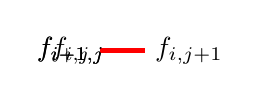
\begin{tikzpicture}
		[parent anchor=east,child anchor=west,grow=east]
		%\tikzstyle{every node}=[ball color=red,circle,text=white]
		\tikzstyle{edge from parent}=[draw,ultra thick,red]
		\node {$f_{i+1,j}$}
		node {$f_{i,j}$}
		child {node {$f_{i,j+1}$}}
		node {$f_{i-1,j}$};
	\end{tikzpicture}
\end{center}

We can treat the equations as a system of linear equations in a matrix form:
%  Here:
%M1 fj−1 =M2 fj
%1−β1 −γ1 0 0 0 0 
%−α1−β−γ 0 0 0 222
%0−α31−β3−γ3 00 M1=0 0 􏰦 􏰦 􏰦 0
%
%0 0 0 −αM−2 1−βM−2 −γM−2 
%0 0 0 0 −α 1−β  M−1 M−1
%1+β1 γ1 0 0 0 0 α1+βγ 0 0 0
%222
%0α31+β3−γ3 00 M2=0 0􏰦􏰦􏰦 0
%
%0 0 0 αM−2 1+βM−2 γM−2  
%0 0 0 0 α 1+β  M−1 M−1
%We can solve for the matrix M on every iterative procedure. [ 109 ]
%f=f ,f ,...,f T i  1,j 2,j M1−1,j

\subsubsection{\texttt{FDCnEu} class}
The \texttt{python} implementation of the Crank-Nicolson method is given in the following \texttt{FDCnEu} class, which inherits from the \texttt{FDExplicitEu} class and overrides the usual methods.

\begin{codebox}
\begin{Verbatim}[commandchars=\\\{\}]
\PY{k}{class} \PY{n+nc}{FDCnEu}\PY{p}{(}\PY{n}{FDExplicitEu}\PY{p}{)}\PY{p}{:}
    \PY{k}{def} \PY{n+nf}{\PYZus{}setup\PYZus{}coefficients\PYZus{}}\PY{p}{(}\PY{n+nb+bp}{self}\PY{p}{)}\PY{p}{:} 
        \PY{n+nb+bp}{self}\PY{o}{.}\PY{n}{alpha} \PY{o}{=} \PY{l+m+mf}{0.25}\PY{o}{*}\PY{n+nb+bp}{self}\PY{o}{.}\PY{n}{dt}\PY{o}{*}\PY{p}{(}\PY{p}{(}\PY{n+nb+bp}{self}\PY{o}{.}\PY{n}{sigma}\PY{o}{*}\PY{o}{*}\PY{l+m+mi}{2}\PY{p}{)}\PY{o}{*}\PY{p}{(}\PY{n+nb+bp}{self}\PY{o}{.}\PY{n}{i\PYZus{}values}\PY{o}{*}\PY{o}{*}\PY{l+m+mi}{2}\PY{p}{)} 
                     \PY{o}{\PYZhy{}} \PY{n+nb+bp}{self}\PY{o}{.}\PY{n}{r}\PY{o}{*}\PY{n+nb+bp}{self}\PY{o}{.}\PY{n}{i\PYZus{}values}\PY{p}{)} 
        \PY{n+nb+bp}{self}\PY{o}{.}\PY{n}{beta} \PY{o}{=} \PY{o}{\PYZhy{}}\PY{n+nb+bp}{self}\PY{o}{.}\PY{n}{dt}\PY{o}{*}\PY{l+m+mf}{0.5}\PY{o}{*}\PY{p}{(}\PY{p}{(}\PY{n+nb+bp}{self}\PY{o}{.}\PY{n}{sigma}\PY{o}{*}\PY{o}{*}\PY{l+m+mi}{2}\PY{p}{)}\PY{o}{*}\PY{p}{(}\PY{n+nb+bp}{self}\PY{o}{.}\PY{n}{i\PYZus{}values}\PY{o}{*}\PY{o}{*}\PY{l+m+mi}{2}\PY{p}{)} 
                    \PY{o}{+} \PY{n+nb+bp}{self}\PY{o}{.}\PY{n}{r}\PY{p}{)}
        \PY{n+nb+bp}{self}\PY{o}{.}\PY{n}{gamma} \PY{o}{=} \PY{l+m+mf}{0.25}\PY{o}{*}\PY{n+nb+bp}{self}\PY{o}{.}\PY{n}{dt}\PY{o}{*}\PY{p}{(}\PY{p}{(}\PY{n+nb+bp}{self}\PY{o}{.}\PY{n}{sigma}\PY{o}{*}\PY{o}{*}\PY{l+m+mi}{2}\PY{p}{)}\PY{o}{*}\PY{p}{(}\PY{n+nb+bp}{self}\PY{o}{.}\PY{n}{i\PYZus{}values}\PY{o}{*}\PY{o}{*}\PY{l+m+mi}{2}\PY{p}{)} 
                     \PY{o}{+} \PY{n+nb+bp}{self}\PY{o}{.}\PY{n}{r}\PY{o}{*}\PY{n+nb+bp}{self}\PY{o}{.}\PY{n}{i\PYZus{}values}\PY{p}{)}
        \PY{n+nb+bp}{self}\PY{o}{.}\PY{n}{M1} \PY{o}{=} \PY{o}{\PYZhy{}}\PY{n}{np}\PY{o}{.}\PY{n}{diag}\PY{p}{(}\PY{n+nb+bp}{self}\PY{o}{.}\PY{n}{alpha}\PY{p}{[}\PY{l+m+mi}{2}\PY{p}{:}\PY{n+nb+bp}{self}\PY{o}{.}\PY{n}{M}\PY{p}{]}\PY{p}{,} \PY{o}{\PYZhy{}}\PY{l+m+mi}{1}\PY{p}{)} 
                  \PY{o}{+} \PY{n}{np}\PY{o}{.}\PY{n}{diag}\PY{p}{(}\PY{l+m+mi}{1}\PY{o}{\PYZhy{}}\PY{n+nb+bp}{self}\PY{o}{.}\PY{n}{beta}\PY{p}{[}\PY{l+m+mi}{1}\PY{p}{:}\PY{n+nb+bp}{self}\PY{o}{.}\PY{n}{M}\PY{p}{]}\PY{p}{)} 
                  \PY{o}{+} \PY{n}{np}\PY{o}{.}\PY{n}{diag}\PY{p}{(}\PY{n+nb+bp}{self}\PY{o}{.}\PY{n}{gamma}\PY{p}{[}\PY{l+m+mi}{1}\PY{p}{:}\PY{n+nb+bp}{self}\PY{o}{.}\PY{n}{M}\PY{o}{\PYZhy{}}\PY{l+m+mi}{1}\PY{p}{]}\PY{p}{,} \PY{l+m+mi}{1}\PY{p}{)}
        \PY{n+nb+bp}{self}\PY{o}{.}\PY{n}{M2} \PY{o}{=} \PY{n}{np}\PY{o}{.}\PY{n}{diag}\PY{p}{(}\PY{n+nb+bp}{self}\PY{o}{.}\PY{n}{alpha}\PY{p}{[}\PY{l+m+mi}{2}\PY{p}{:}\PY{n+nb+bp}{self}\PY{o}{.}\PY{n}{M}\PY{p}{]}\PY{p}{,} \PY{o}{\PYZhy{}}\PY{l+m+mi}{1}\PY{p}{)} 
                  \PY{o}{+} \PY{n}{np}\PY{o}{.}\PY{n}{diag}\PY{p}{(}\PY{l+m+mi}{1}\PY{o}{+}\PY{n+nb+bp}{self}\PY{o}{.}\PY{n}{beta}\PY{p}{[}\PY{l+m+mi}{1}\PY{p}{:}\PY{n+nb+bp}{self}\PY{o}{.}\PY{n}{M}\PY{p}{]}\PY{p}{)} 
                  \PY{o}{+} \PY{n}{np}\PY{o}{.}\PY{n}{diag}\PY{p}{(}\PY{n+nb+bp}{self}\PY{o}{.}\PY{n}{gamma}\PY{p}{[}\PY{l+m+mi}{1}\PY{p}{:}\PY{n+nb+bp}{self}\PY{o}{.}\PY{n}{M}\PY{o}{\PYZhy{}}\PY{l+m+mi}{1}\PY{p}{]}\PY{p}{,} \PY{l+m+mi}{1}\PY{p}{)}
		
    \PY{k}{def} \PY{n+nf}{\PYZus{}traverse\PYZus{}grid\PYZus{}}\PY{p}{(}\PY{n+nb+bp}{self}\PY{p}{)}\PY{p}{:}
        \PY{n}{P}\PY{p}{,} \PY{n}{L}\PY{p}{,} \PY{n}{U} \PY{o}{=} \PY{n}{linalg}\PY{o}{.}\PY{n}{lu}\PY{p}{(}\PY{n+nb+bp}{self}\PY{o}{.}\PY{n}{M1}\PY{p}{)}
        \PY{k}{for} \PY{n}{j} \PY{o+ow}{in} \PY{n+nb}{reversed}\PY{p}{(}\PY{n+nb}{range}\PY{p}{(}\PY{n+nb+bp}{self}\PY{o}{.}\PY{n}{N}\PY{p}{)}\PY{p}{)}\PY{p}{:} 
            \PY{n}{x1} \PY{o}{=} \PY{n}{linalg}\PY{o}{.}\PY{n}{solve}\PY{p}{(}\PY{n}{L}\PY{p}{,} \PY{n}{np}\PY{o}{.}\PY{n}{dot}\PY{p}{(}\PY{n+nb+bp}{self}\PY{o}{.}\PY{n}{M2}\PY{p}{,} \PY{n+nb+bp}{self}\PY{o}{.}\PY{n}{grid}\PY{p}{[}\PY{l+m+mi}{1}\PY{p}{:}\PY{n+nb+bp}{self}\PY{o}{.}\PY{n}{M}\PY{p}{,} \PY{n}{j}\PY{o}{+}\PY{l+m+mi}{1}\PY{p}{]}\PY{p}{)}\PY{p}{)}
            \PY{n}{x2} \PY{o}{=} \PY{n}{linalg}\PY{o}{.}\PY{n}{solve}\PY{p}{(}\PY{n}{U}\PY{p}{,} \PY{n}{x1}\PY{p}{)} 
            \PY{n+nb+bp}{self}\PY{o}{.}\PY{n}{grid}\PY{p}{[}\PY{l+m+mi}{1}\PY{p}{:}\PY{n+nb+bp}{self}\PY{o}{.}\PY{n}{M}\PY{p}{,} \PY{n}{j}\PY{p}{]} \PY{o}{=} \PY{n}{x2}
\end{Verbatim}
\end{codebox}

Using the same examples as with the explicit and implicit methods, we can price an European put option using the Crank-Nicolson method for different time point intervals:

\begin{codebox}
\begin{Verbatim}[commandchars=\\\{\}]
\PY{n}{option} \PY{o}{=} \PY{n}{FDCnEu}\PY{p}{(}\PY{l+m+mi}{50}\PY{p}{,} \PY{l+m+mi}{50}\PY{p}{,} \PY{l+m+mf}{0.1}\PY{p}{,} \PY{l+m+mf}{5.}\PY{o}{/}\PY{l+m+mf}{12.}\PY{p}{,} \PY{l+m+mf}{0.4}\PY{p}{,} \PY{l+m+mi}{100}\PY{p}{,} \PY{l+m+mi}{100}\PY{p}{,} \PY{l+m+mi}{100}\PY{p}{,} \PY{k+kc}{False}\PY{p}{)}
\PY{n+nb}{print} \PY{p}{(}\PY{n}{option}\PY{o}{.}\PY{n}{price}\PY{p}{(}\PY{p}{)}\PY{p}{)}

1.6382715987620217e-10

\PY{n}{option} \PY{o}{=} \PY{n}{FDCnEu}\PY{p}{(}\PY{l+m+mi}{50}\PY{p}{,} \PY{l+m+mi}{50}\PY{p}{,} \PY{l+m+mf}{0.1}\PY{p}{,} \PY{l+m+mf}{5.}\PY{o}{/}\PY{l+m+mf}{12.}\PY{p}{,} \PY{l+m+mf}{0.4}\PY{p}{,} \PY{l+m+mi}{100}\PY{p}{,} \PY{l+m+mi}{100}\PY{p}{,} \PY{l+m+mi}{1000}\PY{p}{,} \PY{k+kc}{False}\PY{p}{)}
\PY{n+nb}{print} \PY{p}{(}\PY{n}{option}\PY{o}{.}\PY{n}{price}\PY{p}{(}\PY{p}{)}\PY{p}{)}

1.0220621095408119e-10
\end{Verbatim}
\end{codebox}

From the observed values, the Crank-Nicolson method not only avoids the instability issue seen in the explicit scheme, but also converges faster than both the explicit and implicit methods. The implicit method requires more iterations, or bigger values of $N$, to produce values close to those of the Crank-Nicolson method.
